% Options for packages loaded elsewhere
\PassOptionsToPackage{unicode}{hyperref}
\PassOptionsToPackage{hyphens}{url}
%
\documentclass[
]{article}
\usepackage{amsmath,amssymb}
\usepackage{lmodern}
\usepackage{iftex}
\usepackage{graphicx}
\ifPDFTeX
  \usepackage[T1]{fontenc}
  \usepackage[utf8]{inputenc}
  \usepackage{textcomp} % provide euro and other symbols
\else % if luatex or xetex
  \usepackage{unicode-math}
  \defaultfontfeatures{Scale=MatchLowercase}
  \defaultfontfeatures[\rmfamily]{Ligatures=TeX,Scale=1}
\fi
% Use upquote if available, for straight quotes in verbatim environments
\IfFileExists{upquote.sty}{\usepackage{upquote}}{}
\IfFileExists{microtype.sty}{% use microtype if available
  \usepackage[]{microtype}
  \UseMicrotypeSet[protrusion]{basicmath} % disable protrusion for tt fonts
}{}
\makeatletter
\@ifundefined{KOMAClassName}{% if non-KOMA class
  \IfFileExists{parskip.sty}{%
    \usepackage{parskip}
  }{% else
    \setlength{\parindent}{0pt}
    \setlength{\parskip}{6pt plus 2pt minus 1pt}}
}{% if KOMA class
  \KOMAoptions{parskip=half}}
\makeatother
\usepackage{xcolor}
\usepackage{longtable,booktabs,array}
\usepackage{calc} % for calculating minipage widths
% Correct order of tables after \paragraph or \subparagraph
\usepackage{etoolbox}
\makeatletter
\patchcmd\longtable{\par}{\if@noskipsec\mbox{}\fi\par}{}{}
\makeatother
% Allow footnotes in longtable head/foot
\IfFileExists{footnotehyper.sty}{\usepackage{footnotehyper}}{\usepackage{footnote}}
\makesavenoteenv{longtable}
\usepackage{graphicx}
\makeatletter
\def\maxwidth{\ifdim\Gin@nat@width>\linewidth\linewidth\else\Gin@nat@width\fi}
\def\maxheight{\ifdim\Gin@nat@height>\textheight\textheight\else\Gin@nat@height\fi}
\makeatother
% Scale images if necessary, so that they will not overflow the page
% margins by default, and it is still possible to overwrite the defaults
% using explicit options in \includegraphics[width, height, ...]{}
\setkeys{Gin}{width=\maxwidth,height=\maxheight,keepaspectratio}
% Set default figure placement to htbp
\makeatletter
\def\fps@figure{htbp}
\makeatother
\setlength{\emergencystretch}{3em} % prevent overfull lines
\providecommand{\tightlist}{%
  \setlength{\itemsep}{0pt}\setlength{\parskip}{0pt}}
\setcounter{secnumdepth}{-\maxdimen} % remove section numbering
\ifLuaTeX
  \usepackage{selnolig}  % disable illegal ligatures
\fi
\IfFileExists{bookmark.sty}{\usepackage{bookmark}}{\usepackage{hyperref}}
\IfFileExists{xurl.sty}{\usepackage{xurl}}{} % add URL line breaks if available
\urlstyle{same} % disable monospaced font for URLs
\hypersetup{
  hidelinks,
  pdfcreator={LaTeX via pandoc}}

\author{Darshan Odedara}
\date{}


\begin{document}

\begin{center}
{\LARGE \textbf{Traveling Salesman Problem Using Ant Colony Optimization Algorithm}} \\
{\LARGE \textbf{(ACO - TSP)}}
\end{center}

\vspace{3cm}

\textbf{1. Abstract}

The Traveling Salesman Problem (TSP) stands as one of the most iconic
and challenging optimization problems in computer science and operations
research. At its core, the TSP involves finding the shortest possible
route for a salesman who must visit a set of cities exactly once and
return to the starting point. While deceptively simple in its
formulation, the TSP\textquotesingle s complexity grows exponentially
with the number of cities, making it a quintessential NP-hard problem
that has captivated researchers and practitioners for decades.

Traditional approaches to solving the TSP, such as brute-force
enumeration or dynamic programming, quickly become impractical as the
problem size increases. The factorial growth in the number of possible
solutions renders these methods computationally infeasible for all but
the smallest instances. This limitation has spurred the development of
numerous heuristic and metaheuristic algorithms aimed at finding
near-optimal solutions within reasonable time frames.

Among these innovative approaches, the Ant Colony Optimization (ACO)
algorithm has emerged as a particularly promising and fascinating
method. Inspired by the foraging behavior of ant colonies in nature, ACO
represents a paradigm shift in optimization techniques. It leverages the
concept of swarm intelligence, where simple agents (artificial ants)
collaboratively solve complex problems through indirect communication.

This project delves deep into the implementation and analysis of the ACO
algorithm for solving the Traveling Salesman Problem. The core mechanism
of ACO revolves around the simulation of pheromone trails left by ants
as they traverse paths between cities. These pheromone trails serve as a
form of distributed memory, influencing the path choices of subsequent
ants. Over time, this process leads to the emergence of optimal or
near-optimal routes.

Our implementation incorporates several key components of the ACO
algorithm:

\begin{enumerate}
\def\labelenumi{\arabic{enumi}.}
\item
  Graph Representation: We model the TSP as a complete weighted graph,
  where nodes represent cities and edges represent the distances between
  them.
\item
  Ant Movement Simulation: Artificial ants construct tours by
  probabilistically choosing their next destination based on pheromone
  levels and heuristic information (typically the inverse of the
  distance).
\item
  Pheromone Update Mechanism: After each iteration, pheromone levels on
  edges are updated. This involves both evaporation (to prevent
  premature convergence) and deposition (to reinforce promising paths).
\item
  Solution Construction and Improvement: The algorithm iteratively
  builds and refines solutions, gradually converging towards optimal or
  near-optimal tours.
\end{enumerate}

Our study encompasses a comprehensive evaluation of the ACO
algorithm\textquotesingle s performance across various TSP instances,
ranging from small-scale problems to large, complex scenarios. We
analyze the algorithm\textquotesingle s efficiency in terms of solution
quality and computational time, comparing its performance against
traditional methods and other metaheuristics.

Furthermore, we explore parameter tuning and algorithmic enhancements to
improve the ACO\textquotesingle s effectiveness. This includes
investigating different pheromone update rules, incorporating local
search procedures, and experimenting with hybrid approaches that combine
ACO with other optimization techniques.

The results of our implementation demonstrate the robustness and
adaptability of the ACO algorithm in tackling the TSP. We observe that
for large problem instances, ACO consistently outperforms classical
methods, providing high-quality solutions within reasonable
computational bounds. However, we also note that for smaller instances,
simpler heuristics may sometimes offer comparable or superior
performance.

This project not only contributes to the practical application of ACO in
solving TSPs but also provides insights into the broader field of swarm
intelligence and its potential in addressing complex optimization
challenges. The findings have implications beyond the TSP, suggesting
avenues for applying similar bio-inspired algorithms to other NP-hard
problems in logistics, scheduling, and network optimization.

In conclusion, our implementation and analysis of the Ant Colony
Optimization algorithm for the Traveling Salesman Problem showcase the
power of nature-inspired computing in tackling one of the most enduring
challenges in combinatorial optimization. The project underscores the
potential of swarm intelligence approaches in finding efficient
solutions to complex problems, paving the way for further research and
applications in this exciting field.

\textbf{2. Introduction}

The Traveling Salesman Problem (TSP) stands as a cornerstone in the
realm of combinatorial optimization, captivating researchers and
practitioners across various disciplines for decades. At its core, the
TSP presents a deceptively simple challenge: given a list of cities and
the distances between each pair of cities, the task is to find the
shortest possible route that visits each city exactly once and returns
to the origin city. This problem, while easy to state, harbors a
complexity that grows exponentially with the number of cities, making it
a quintessential example of an NP-hard problem in computational theory.

The significance of the TSP extends far beyond its theoretical intrigue.
Its practical applications permeate numerous domains, including
logistics, manufacturing, and telecommunications. In logistics,
efficient routing of delivery vehicles can lead to substantial cost
savings and reduced environmental impact. In manufacturing, optimizing
the movement of robotic arms in circuit board assembly can significantly
increase production efficiency. The problem also finds relevance in DNA
sequencing, computer wiring, and even in planning interplanetary
spacecraft trajectories.

The historical pursuit of solving the TSP has been marked by significant
milestones in algorithm development and computational techniques. Early
approaches relied on brute-force enumeration, which quickly became
impractical as problem sizes grew. The development of dynamic
programming and branch-and-bound algorithms in the mid-20th century
provided more efficient exact methods, but these too faltered in the
face of large-scale problems. This limitation spurred the development of
heuristic and metaheuristic approaches, aimed at finding near-optimal
solutions within reasonable time frames.

Among the myriad of approaches developed to tackle the TSP, the Ant
Colony Optimization (ACO) algorithm represents a paradigm shift in
problem-solving methodology. Introduced by Marco Dorigo in the early
1990s, ACO draws inspiration from the foraging behavior of ant colonies
in nature. The algorithm\textquotesingle s core idea is brilliantly
simple yet profoundly effective: simulate the behavior of ants leaving
pheromone trails as they search for food, using these trails to
communicate indirectly and collectively solve complex problems.

The ACO approach to the TSP works as follows: artificial ants are
deployed to construct tours through the cities. As they move, they
deposit pheromones on the edges they traverse. The amount of pheromone
deposited is typically inversely proportional to the tour length,
meaning shorter tours receive more pheromone. Subsequent ants are then
more likely to follow edges with higher pheromone concentrations. Over
time, this positive feedback mechanism leads to the emergence of shorter
tours.

What makes ACO particularly intriguing is its ability to balance
exploration and exploitation. The probabilistic nature of ant movement
allows for continuous exploration of the solution space, while the
pheromone update mechanism intensifies the search in promising areas.
This balance helps ACO avoid getting trapped in local optima, a common
pitfall for many optimization algorithms.

The implementation of ACO for the TSP involves several key components:

\begin{enumerate}
\def\labelenumi{\arabic{enumi}.}
\item
  Graph Representation: The problem is modeled as a complete graph where
  nodes represent cities and edges represent paths between cities.
\item
  Ant Tour Construction: Ants build tours by probabilistically choosing
  their next city based on pheromone levels and heuristic information
  (typically the inverse of the distance).
\item
  Pheromone Update: After all ants complete their tours, pheromone
  levels are updated. This involves evaporation (to prevent stagnation)
  and deposition (to reinforce good paths).
\item
  Iterative Improvement: The process is repeated over multiple
  iterations, gradually improving the quality of solutions.
\end{enumerate}

The effectiveness of ACO in solving the TSP has been demonstrated across
numerous studies, often outperforming traditional heuristics for large
problem instances. Its success has led to various enhancements and
hybrid approaches, combining ACO with local search techniques or other
metaheuristics to further improve performance.

This project aims to delve deep into the implementation and analysis of
the ACO algorithm for solving the TSP. We will explore the intricacies
of the algorithm\textquotesingle s design, investigate parameter tuning
for optimal performance, and conduct comprehensive evaluations across
various problem instances. By comparing ACO\textquotesingle s
performance against other established methods, we seek to provide
insights into its strengths and limitations.

Moreover, our study will extend beyond mere implementation to explore
potential enhancements and modifications to the basic ACO framework.
This includes investigating different pheromone update rules,
incorporating local search procedures, and experimenting with parallel
implementations to leverage modern computing architectures.

The insights gained from this project have implications that reach
beyond the TSP. The principles underlying ACO -- decentralized
decision-making, indirect communication through environment
modification, and emergent behavior -- have potential applications in a
wide array of complex optimization problems. From network routing and
scheduling to machine learning and artificial intelligence, the concepts
explored in this study could pave the way for innovative solutions in
diverse fields.

As we embark on this exploration of Ant Colony Optimization for the
Traveling Salesman Problem, we aim not only to contribute to the
practical application of this fascinating algorithm but also to deepen
our understanding of swarm intelligence and its potential in solving
some of the most challenging problems in computational science and
engineering.

\textbf{3. Problem Statement}

The Traveling Salesman Problem (TSP) represents one of the most
intensively studied challenges in combinatorial optimization, serving as
a benchmark for algorithmic efficiency and a proxy for a wide array of
real-world optimization scenarios. At its core, the TSP asks a
deceptively simple question: given a list of cities and the distances
between each pair of cities, what is the shortest possible route that
visits each city exactly once and returns to the origin city?

The complexity of the TSP lies in its combinatorial nature. For n
cities, there are (n-1)! possible routes to consider. This factorial
growth in the number of potential solutions renders brute-force
approaches impractical for all but the smallest instances. For example,
a problem with just 20 cities has over 1018 possible routes -- a number
so large that even the fastest computers would take years to evaluate
every possibility.

This exponential growth in complexity classifies the TSP as an NP-hard
problem, placing it among the most challenging problems in computer
science. The significance of NP-hard problems extends beyond academia;
they represent a class of problems for which no known polynomial-time
algorithms exist. This means that as the problem size increases, the
time required to solve it grows at a rate faster than any polynomial
function.

The practical implications of the TSP\textquotesingle s complexity are
profound and far-reaching. In logistics and supply chain management,
even marginal improvements in route optimization can translate to
significant cost savings and reduced environmental impact. For instance,
a delivery company optimizing routes for a fleet of vehicles across
hundreds of destinations faces a problem analogous to multiple
interconnected TSPs. The ability to find near-optimal solutions quickly
can lead to reduced fuel consumption, lower operating costs, and
improved service levels.

In manufacturing, the TSP finds applications in processes such as drill
route optimization for printed circuit boards (PCBs). Here, minimizing
the travel distance of the drill head directly impacts production speed
and energy consumption. Similarly, in robotics, optimizing the movement
path for tasks like welding or assembly can significantly enhance
production efficiency.

The challenge posed by the TSP extends beyond its direct applications.
It serves as a prototype for a wide array of optimization problems in
fields as diverse as genetics (DNA sequencing), telecommunications
(network design), and even astronomy (telescope scheduling). The
algorithmic insights gained from tackling the TSP often have broader
implications, informing approaches to other complex optimization
challenges.

Traditional exact methods for solving the TSP, such as branch-and-bound
algorithms or dynamic programming, become computationally infeasible for
large problem instances. This limitation has spurred the development of
heuristic and metaheuristic approaches aimed at finding near-optimal
solutions within reasonable time frames. However, these approaches often
face their own challenges:

\begin{enumerate}
\def\labelenumi{\arabic{enumi}.}
\item
  Solution Quality vs. Computation Time Trade-off: Faster algorithms may
  produce lower-quality solutions, while methods that consistently find
  near-optimal solutions may require prohibitive computation times for
  large instances.
\item
  Scalability: Many algorithms that perform well on small to
  medium-sized problems struggle to maintain their effectiveness as the
  problem size increases.
\item
  Premature Convergence: Some heuristic methods tend to converge too
  quickly to suboptimal solutions, failing to adequately explore the
  solution space.
\item
  Parameter Sensitivity: Many advanced algorithms require careful tuning
  of multiple parameters, which can be problem-specific and
  time-consuming.
\item
  Balancing Exploration and Exploitation: Achieving the right balance
  between exploring new solutions and exploiting known good solutions is
  a persistent challenge in optimization algorithms.
\end{enumerate}

In this context, the Ant Colony Optimization (ACO) algorithm emerges as
a promising approach to addressing these challenges. Inspired by the
foraging behavior of ants, ACO offers a unique perspective on
problem-solving that aligns well with the structure of the TSP. The
algorithm\textquotesingle s decentralized nature, ability to balance
exploration and exploitation, and capacity for parallel implementation
make it particularly suited for tackling large-scale TSP instances.

However, implementing ACO for the TSP is not without its own set of
challenges:

\begin{enumerate}
\def\labelenumi{\arabic{enumi}.}
\item
  Algorithm Design: Crafting an effective implementation requires
  careful consideration of various components, including pheromone
  initialization, update rules, and tour construction mechanisms.
\item
  Parameter Tuning: The performance of ACO can be highly sensitive to
  parameter settings, necessitating a systematic approach to finding
  optimal configurations.
\item
  Computational Efficiency: While ACO can provide high-quality
  solutions, ensuring its computational efficiency, especially for large
  problem instances, remains a key challenge.
\item
  Hybridization: Exploring ways to combine ACO with other optimization
  techniques or local search methods to enhance its performance presents
  both opportunities and complexities.
\item
  Theoretical Analysis: Developing a deeper theoretical understanding of
  ACO\textquotesingle s behavior, convergence properties, and
  performance bounds is an ongoing area of research.
\end{enumerate}

This project aims to address these challenges head-on, implementing and
analyzing the ACO algorithm for solving the TSP. Our goal is not only to
develop an efficient and effective implementation but also to contribute
to the broader understanding of how swarm intelligence approaches can be
leveraged to tackle complex combinatorial optimization problems.

By focusing on the TSP through the lens of Ant Colony Optimization, we
seek to push the boundaries of what\textquotesingle s possible in
solving NP-hard problems, potentially opening new avenues for addressing
a wide range of real-world optimization challenges. The insights gained
from this study have the potential to inform not only future TSP
solutions but also approaches to related problems in logistics,
scheduling, network design, and beyond.

\textbf{4. Scope}

The scope of this project encompasses a comprehensive exploration of the
Ant Colony Optimization (ACO) algorithm as applied to the Traveling
Salesman Problem (TSP). Our aim is to provide a thorough implementation,
analysis, and evaluation of ACO in the context of solving various TSP
instances. The project\textquotesingle s scope can be delineated into
several key areas:

\begin{enumerate}
\def\labelenumi{\arabic{enumi}.}
\item
  Literature Review and Theoretical Foundation Our project begins with
  an extensive review of existing literature on both the Traveling
  Salesman Problem and Ant Colony Optimization. This review will cover:

  \begin{itemize}
  \item
    Historical development of TSP solving methods
  \item
    Fundamental principles and variations of ACO algorithms
  \item
    State-of-the-art approaches in applying ACO to TSP
  \item
    Comparative studies of ACO against other heuristic and metaheuristic
    methods
  \end{itemize}
\end{enumerate}

This foundational work will ensure our implementation is grounded in the
latest research and best practices in the field.

\begin{enumerate}
\def\labelenumi{\arabic{enumi}.}
\setcounter{enumi}{1}
\item
  Algorithm Design and Implementation The core of our project involves
  the detailed design and coding of the ACO algorithm tailored
  specifically for the TSP. This encompasses:

  \begin{itemize}
  \item
    Developing a robust graph representation of the TSP
  \item
    Implementing the ant tour construction mechanism
  \item
    Designing efficient pheromone update rules
  \item
    Creating mechanisms for parameter adjustment and tuning
  \item
    Optimizing the code for performance, considering both time and space
    complexity
  \end{itemize}
\end{enumerate}

We will implement the algorithm in a high-level programming language,
with a focus on modularity and extensibility to facilitate future
enhancements and modifications.

\begin{enumerate}
\def\labelenumi{\arabic{enumi}.}
\setcounter{enumi}{2}
\item
  Experimental Setup and Benchmark Suite To rigorously evaluate our ACO
  implementation, we will create a comprehensive test suite comprising:

  \begin{itemize}
  \item
    A diverse set of TSP instances, ranging from small (10-20 cities) to
    large (1000+ cities)
  \item
    Both symmetric and asymmetric TSP variants
  \item
    Well-known benchmark problems from TSPLIB and other standard sources
  \item
    Custom-generated problem instances to test specific aspects of the
    algorithm
  \end{itemize}
\end{enumerate}

This suite will serve as a standardized testbed for assessing the
performance and scalability of our implementation.

\begin{enumerate}
\def\labelenumi{\arabic{enumi}.}
\setcounter{enumi}{3}
\item
  Performance Analysis and Comparative Study A key component of our
  project is the rigorous analysis of ACO\textquotesingle s performance.
  This will include:

  \begin{itemize}
  \item
    Measuring solution quality (tour length) across different problem
    sizes and types
  \item
    Analyzing computational efficiency in terms of time and memory usage
  \item
    Investigating the algorithm\textquotesingle s scalability as problem
    size increases
  \item
    Comparing ACO\textquotesingle s performance against other methods,
    including:

    \begin{itemize}
    \item
      Exact methods (for small instances)
    \item
      Traditional heuristics (e.g., nearest neighbor, 2-opt)
    \item
      Other metaheuristics (e.g., Genetic Algorithms, Simulated
      Annealing)
    \end{itemize}
  \end{itemize}
\end{enumerate}

We will use statistical methods to ensure the robustness and
significance of our findings.

\begin{enumerate}
\def\labelenumi{\arabic{enumi}.}
\setcounter{enumi}{4}
\item
  Parameter Tuning and Sensitivity Analysis Understanding the impact of
  various parameters on ACO\textquotesingle s performance is crucial.
  Our scope includes:

  \begin{itemize}
  \item
    Systematic exploration of parameter spaces (e.g., number of ants,
    pheromone evaporation rate)
  \item
    Developing methodologies for automatic parameter tuning
  \item
    Analyzing the algorithm\textquotesingle s sensitivity to parameter
    changes across different problem instances
  \end{itemize}
\end{enumerate}

\begin{enumerate}
\def\labelenumi{\arabic{enumi}.}
\setcounter{enumi}{5}
\item
  Algorithm Enhancements and Hybridization Our project scope extends to
  exploring potential improvements and variations of the basic ACO
  algorithm:

  \begin{itemize}
  \item
    Implementing and testing different ACO variants (e.g., MAX-MIN Ant
    System, Ant Colony System)
  \item
    Incorporating local search procedures to enhance solution quality
  \item
    Exploring hybridization with other metaheuristics (e.g., combining
    ACO with Genetic Algorithms or Simulated Annealing)
  \item
    Investigating parallel and distributed implementations to leverage
    multi-core and cluster computing environments
  \end{itemize}
\item
  Visualization and User Interface To aid in understanding and analysis,
  we will develop visualization tools:

  \begin{itemize}
  \item
    Graphical representation of TSP instances and solutions
  \item
    Real-time visualization of ant movements and pheromone trail
    evolution
  \item
    Interactive interface for parameter adjustment and algorithm control
  \item
    Comprehensive reporting and charting of performance metrics
  \end{itemize}
\item
  Real-world Applications and Case Studies While our primary focus is on
  benchmark TSP instances, we will also explore real-world applications:

  \begin{itemize}
  \item
    Collaborating with local logistics companies to test our
    implementation on actual routing problems
  \item
    Developing case studies in areas such as PCB drilling, warehouse
    order picking, or delivery route optimization
  \item
    Analyzing the practical impact of our optimizations in terms of cost
    savings and efficiency improvements
  \end{itemize}
\item
  Theoretical Analysis and Contributions Beyond practical
  implementation, our scope includes theoretical investigations:

  \begin{itemize}
  \item
    Analyzing the convergence properties of our ACO implementation
  \item
    Developing bounds on solution quality and runtime for different
    problem classes
  \item
    Investigating the relationship between problem structure and
    algorithm performance
  \item
    Contributing to the theoretical understanding of
    ACO\textquotesingle s behavior on TSP and related problems
  \end{itemize}
\item
  Documentation and Knowledge Dissemination Comprehensive documentation
  is a crucial part of our project scope:

  \begin{itemize}
  \item
    Detailed technical documentation of the algorithm implementation
  \item
    User manuals for running experiments and interpreting results
  \item
    Academic paper(s) summarizing our findings and contributions
  \item
    Open-source release of our implementation to facilitate further
    research and applications
  \end{itemize}
\item
  Ethical Considerations and Limitations We will address the ethical
  implications and limitations of our work:

  \begin{itemize}
  \item
    Discussing the environmental impact of optimized routing in
    transportation
  \item
    Analyzing potential job market effects of highly optimized logistics
  \item
    Acknowledging the limitations of our approach, including problem
    sizes and types where ACO may not be the best solution
  \end{itemize}
\item
  Future Work and Research Directions Finally, our scope includes
  identifying and outlining potential areas for future research:

  \begin{itemize}
  \item
    Proposing modifications to ACO for handling dynamic or stochastic
    TSP variants
  \item
    Suggesting approaches for applying our insights to other
    combinatorial optimization problems
  \item
    Outlining potential interdisciplinary applications of ACO in fields
    such as bioinformatics or network science
  \end{itemize}
\end{enumerate}

This comprehensive scope ensures that our project not only implements
and analyzes the ACO algorithm for TSP but also contributes
significantly to the broader field of combinatorial optimization and
swarm intelligence. By addressing theoretical foundations, practical
implementations, real-world applications, and future research
directions, our work aims to provide a valuable resource for both
academics and practitioners in the field of optimization and
computational intelligence.


\textbf{5. Related work --}

\textbf{Related Work Around ACO}

Ant Colony Optimization, first introduced by Marco Dorigo in the early
1990s, has been extensively studied for optimization problems,
especially combinatorial problems like the Traveling Salesman Problem
(TSP). Related works often focus on improving the basic ACO algorithm,
hybridizing it with other algorithms, or applying it to new domains.
Some of the key areas include:

\begin{itemize}
\item
  \textbf{Heuristic Improvements}: Researchers have explored variations
  of ACO to speed up convergence and reduce computational cost,
  including enhancements like \emph{Ant Colony System (ACS)},
  \emph{MAX-MIN Ant System (MMAS)}, and \emph{Rank-based Ant System
  (ASrank)}.
\item
  \textbf{Hybrid ACO Approaches}: ACO has been combined with other
  optimization techniques like Genetic Algorithms (GA), Particle Swarm
  Optimization (PSO), or Simulated Annealing (SA) to create more robust
  hybrid algorithms. These hybrids aim to overcome the limitations of
  individual algorithms by leveraging their strengths.
\item
  \textbf{Parallelization}: Given the computational intensity of ACO for
  large problems, parallel ACO versions using modern computing
  architectures (like GPUs, multi-core processors) have been developed
  to speed up the process.
\item
  \textbf{Dynamic and Stochastic Optimization}: ACO has also been
  adapted for dynamic and stochastic problems, where the environment
  changes over time or is uncertain. This includes applications in
  real-time systems like network routing.
\end{itemize}

\textbf{2. Real-World Implementations and Significant Impacts}

ACO has been applied to a variety of real-world problems where
optimization is crucial. Here are some areas where it has made a
significant impact:

\textbf{a. Network Routing and Load Balancing}

One of the most successful real-world applications of ACO is in
\textbf{network routing} and \textbf{load balancing}. The dynamic,
distributed nature of ACO is well-suited for finding optimal paths in
communication networks. ACO-based algorithms have been applied to:

\begin{itemize}
\item
  \textbf{Telecommunications and Internet Routing}: ACO has been used
  for \textbf{adaptive routing} in telecommunication networks to find
  the shortest paths and balance the load in packet-switched networks.
  Examples include algorithms for \textbf{mobile ad-hoc networks
  (MANETs)} and \textbf{wireless sensor networks (WSNs)}.
\item
  \textbf{Data Center Load Balancing}: ACO algorithms have been used for
  balancing traffic loads across servers in large data centers to
  improve efficiency and reduce response times.
\end{itemize}

\textbf{b. Transportation and Logistics}

\begin{itemize}
\item
  \textbf{Vehicle Routing Problem (VRP)}: ACO has been applied to
  optimize delivery routes for logistics companies, solving real-world
  routing problems for fleets of vehicles delivering goods to multiple
  locations. This helps minimize delivery times, fuel consumption, and
  costs.
\item
  \textbf{Supply Chain Optimization}: ACO has been used to improve
  decision-making processes in supply chains, such as inventory
  management, supplier selection, and distribution.
\end{itemize}

\textbf{c. Robotics and Autonomous Systems}

ACO has been successfully applied to \textbf{multi-robot systems} for
path planning, task allocation, and swarm robotics. In this domain,
robots mimic the behavior of ants to achieve tasks like exploration,
object transportation, or coverage of an area. The algorithm helps in
finding optimal paths for robots to navigate through unknown or dynamic
environments.

\textbf{d. Bioinformatics and Protein Folding}

In bioinformatics, ACO has been employed for complex problems like
\textbf{protein folding}, where the objective is to predict the 3D
structure of a protein based on its amino acid sequence.
ACO\textquotesingle s capability to search large solution spaces makes
it effective for these kinds of computational biology problems.

\textbf{e. Industrial Optimization}

\begin{itemize}
\item
  \textbf{Manufacturing Process Optimization}: ACO has been used to
  optimize job scheduling in manufacturing plants, improving efficiency
  in processes such as assembly lines.
\item
  \textbf{Circuit Design}: The algorithm has been applied to
  \textbf{VLSI design} for optimizing layouts of circuits on silicon
  chips.
\end{itemize}

\textbf{3. Ongoing Research Around ACO}

There is ongoing research aimed at improving ACO\textquotesingle s
performance and extending its applications. Some current trends include:

\textbf{a. Hybridization with Deep Learning}

Researchers are exploring hybrid approaches where ACO is combined with
\textbf{deep learning} techniques. For instance, ACO can be used for
\textbf{feature selection} in machine learning tasks, helping to reduce
the dimensionality of data before feeding it into deep learning models.
The hybridization is aimed at improving optimization in neural network
training or in reinforcement learning tasks.

\textbf{b. Adaptive and Self-Tuning ACO}

Recent research is focusing on \textbf{adaptive ACO algorithms} where
the parameters (such as pheromone evaporation rate or the influence of
pheromone) are adjusted dynamically based on the
problem\textquotesingle s current state. This helps ACO better adapt to
different problem instances without requiring manual tuning.

\textbf{c. Applications in Smart Cities}

ACO is being researched in the context of \textbf{smart cities} for
optimizing \textbf{traffic management systems}, \textbf{waste collection
routes}, and \textbf{urban planning}. These applications benefit from
ACO's ability to find optimal solutions in complex, dynamic
environments.

\textbf{d. Quantum ACO}

Researchers are investigating \textbf{quantum versions of ACO} to
leverage the principles of quantum computing. This involves using
quantum-inspired operators for better exploration of the solution space,
potentially leading to breakthroughs in solving NP-hard problems like
TSP more efficiently.

\textbf{e. Multi-Objective ACO}

Recent efforts have also gone into \textbf{multi-objective optimization}
using ACO, where multiple conflicting objectives (like cost, time, and
quality) are optimized simultaneously. This is especially useful in
fields like \textbf{project scheduling} and \textbf{engineering design},
where trade-offs must be managed.

\textbf{f. Security and Cryptography}

In cybersecurity, ACO is being explored for \textbf{intrusion detection
systems} (IDS) and \textbf{cryptography}. The algorithm can help detect
abnormal patterns in network traffic, helping in the development of more
robust security systems.

\textbf{Conclusion}

Ant Colony Optimization has matured into a powerful algorithm with
diverse applications ranging from telecommunications to bioinformatics.
The ongoing research is focused on improving its efficiency through
hybrid algorithms, parallelization, and adaptive techniques. New domains
such as quantum computing and smart cities continue to emerge as
exciting areas where ACO can make a significant impact.

\textbf{6. Design}

This section will provide a detailed technical overview of how you plan
to structure and implement your ACO algorithm for solving TSP.
We\textquotesingle ll cover the following subsections:

\begin{enumerate}
\def\labelenumi{\arabic{enumi}.}
\item
  \textbf{Overall Architecture}
\item
  \textbf{Interfaces Defined}
\item
  \textbf{Class Diagrams}
\end{enumerate}

\textbf{a. Overall Architecture}

The overall architecture of your ACO solution for TSP consists of
several steps:

\textbf{1. Initialization Phase:}

\begin{itemize}
\item
  \textbf{Parameters Setup}: Define and initialize the parameters such
  as:

  \begin{itemize}
  \item
    Number of ants (m)
  \item
    Number of cities (n)
  \item
    Pheromone matrix ($\tau$): Tracks the pheromone levels on each edge.
  \item
    Visibility ($\eta$): Inverse of distance between cities (i.e., how
    attractive a city is to visit).
  \item
    Alpha ($\alpha$): Controls the influence of pheromone in the
    decision-making process.
  \item
    Beta ($\beta$): Controls the influence of the distance (visibility) in the
    decision-making process.
  \item
    Pheromone evaporation rate ($\rho$): Controls how fast pheromone
    evaporates over time.
  \end{itemize}
\end{itemize}

\textbf{2. Solution Construction by Ants:}

\begin{itemize}
\item
  Each ant starts from a randomly selected city.
\item
  At each step, an ant chooses the next city to visit based on a
  \textbf{probabilistic rule}, which depends on:

  \begin{itemize}
  \item
    The amount of pheromone on the path to that city.
  \item
    The inverse of the distance to that city (visibility).
  \end{itemize}
\item
  This process repeats until all cities have been visited.
\end{itemize}

The formula for choosing the next city j from the current city i is:

\begin{figure}[htbp]
\centering
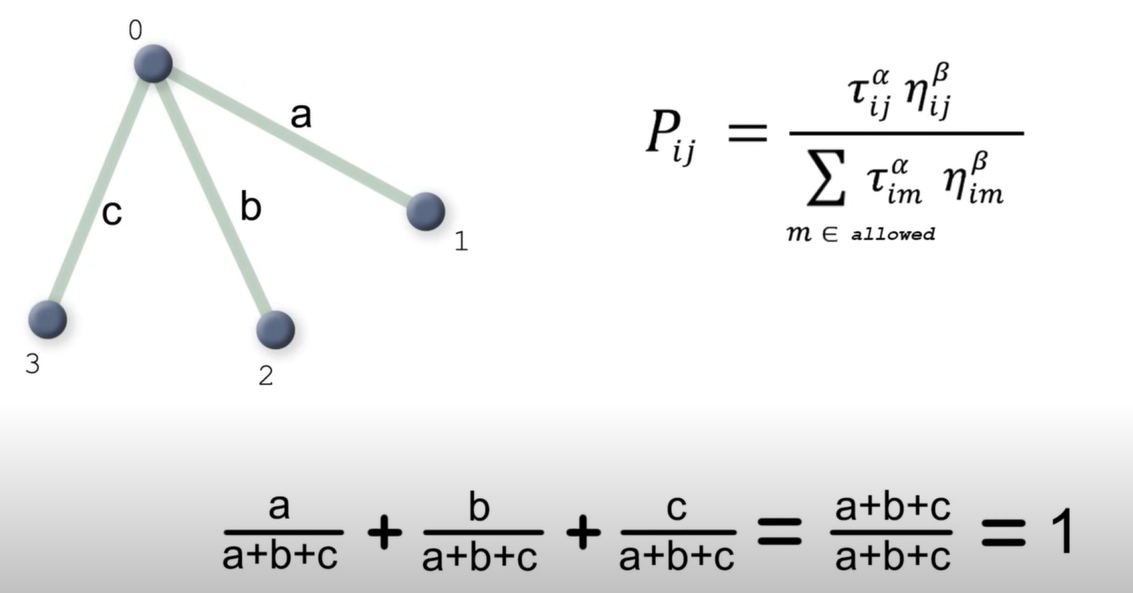
\includegraphics[width=6.26806in,height=2.24074in]{vertopal_760f295f834e4c75be83813a3300ccd6/media/image1.png}
\caption{Formula for calculating the probability that an ant will take a certain path. \label{fig:my_label}}
\end{figure}

Where:

\begin{itemize}
\item
  $\tau_{ij}$\hspace{0pt} is the pheromone level on the edge from city i to city
  j.
\item
  $\eta_{ij}$\hspace{0pt} is the visibility (1/distance) between city i and city
  j.
\item
  The denominator is the sum over all possible cities k that the ant
  has not visited yet.
\end{itemize}

\textbf{3. Pheromone Update:}

\begin{itemize}
\item
  After all ants complete their tours, the pheromone levels on the edges
  are updated.

  \begin{itemize}
  \item
    \textbf{Evaporation}: Reduce the pheromone level by a factor (1 - $\rho$).
  \item
    \textbf{Pheromone deposit}: Increase the pheromone on the edges that
    were used by the best ants.
  \end{itemize}
\end{itemize}

The formula for updating the pheromone is:

\begin{figure}[htbp]
\centering
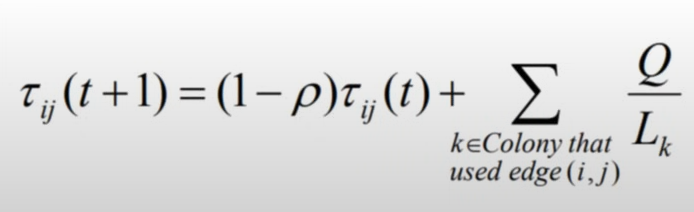
\includegraphics[width=5in,height=1.5in]{vertopal_760f295f834e4c75be83813a3300ccd6/media/image2.png}
\caption{Formula to update Pheromone on path i to j after each iteration. {\label{fig:my_label}}}
\end{figure}

Where:

\begin{itemize}
\item
  $L_{k}$ is the length of the tour for ant k.
\item
  Q is a constant (total pheromone quantity).
\item
  The sum is over all ants that used the edge (i,j) in their tour.
\end{itemize}

\textbf{4. Stopping Criterion:}

\begin{itemize}
\item
  The process repeats for a predefined number of iterations or until the
  solution converges (i.e., no significant improvement in the best
  solution found).
\end{itemize}

\textbf{5. Output:}

\begin{itemize}
\item
  Once the algorithm completes, it outputs the best path (tour) found
  and the corresponding distance.
\end{itemize}

\textbf{Architecture Diagram}:

\begin{itemize}
\item
  A high-level architecture diagram could depict the interactions
  between different components:

  \begin{itemize}
  \item
    \textbf{ACO Controller}: Manages the initialization, solution
    construction, and pheromone updates.
  \item
    \textbf{Ants}: Represent agents that traverse the graph.
  \item
    \textbf{Pheromone Matrix}: A 2D array that stores pheromone levels.
  \item
    \textbf{TSP Graph}: Represents cities and the distances between
    them.
  \end{itemize}
\end{itemize}

\textbf{b. Interfaces Defined}

This section will define the key modules or functions in the system and
their interfaces:

\begin{enumerate}
\def\labelenumi{\arabic{enumi}.}
\item
  \textbf{ACO (Ant Colony Optimization) Module}

  \begin{itemize}
  \item
    \textbf{initialize\_parameters(n, m, $\alpha$, $\beta$, $\rho$, Q)}: Initializes the
    parameters for the algorithm.

    \begin{itemize}
    \item
      Input: Number of cities (n), number of ants (m), parameters $\alpha$, $\beta$,
      $\rho$, Q.
    \item
      Output: Initialized pheromone matrix and other relevant data.
    \end{itemize}
  \item
    \textbf{run\_aco(iterations)}: Runs the ACO algorithm for a given
    number of iterations.

    \begin{itemize}
    \item
      Input: Number of iterations.
    \item
      Output: Best solution found (tour and total distance).
    \end{itemize}
  \end{itemize}
\item
  \textbf{Ant Module}

  \begin{itemize}
  \item
    \textbf{choose\_next\_city(allowed\_cities, current\_city,
    pheromone\_matrix, visibility, $\alpha$, $\beta$)}: Selects the next city based
    on pheromone levels and visibility.

    \begin{itemize}
    \item
      Input: List of allowed cities, current city, pheromone matrix,
      visibility matrix, parameters $\alpha$ and $\beta$.
    \item
      Output: The next city to visit.
    \end{itemize}
  \item
    \textbf{calculate\_tour\_length(tour)}: Calculates the total length
    of the ant\textquotesingle s tour.

    \begin{itemize}
    \item
      Input: List of cities visited by the ant (tour).
    \item
      Output: Total distance of the tour.
    \end{itemize}
  \end{itemize}
\item
  \textbf{Pheromone Update Module}

  \begin{itemize}
  \item
    \textbf{evaporate\_pheromones(pheromone\_matrix, $\rho$)}: Evaporates
    pheromones from all edges.

    \begin{itemize}
    \item
      Input: Pheromone matrix, evaporation rate $\rho$.
    \item
      Output: Updated pheromone matrix.
    \end{itemize}
  \item
    \textbf{update\_pheromones(pheromone\_matrix, ant\_solutions, Q)}:
    Deposits pheromones on the edges used by the ants.

    \begin{itemize}
    \item
      Input: Pheromone matrix, list of ant solutions (tours), total
      pheromone quantity QQQ.
    \item
      Output: Updated pheromone matrix.
    \end{itemize}
  \end{itemize}
\item
  \textbf{TSP Graph Module}

  \begin{itemize}
  \item
    \textbf{generate\_cities(n)}: Generates a set of cities (and their
    coordinates).

    \begin{itemize}
    \item
      Input: Number of cities nnn.
    \item
      Output: List of cities with coordinates.
    \end{itemize}
  \item
    \textbf{calculate\_distances(cities)}: Computes the distance between
    every pair of cities.

    \begin{itemize}
    \item
      Input: List of cities with coordinates.
    \item
      Output: A 2D matrix representing distances between each pair of
      cities.
    \end{itemize}
  \end{itemize}
\end{enumerate}

\textbf{c. Class Diagrams}

\href{https://github.com/darsh0711/AI-DA2}{\textit{(Link to Github repo)}}


The class diagram provides a visual overview of how the components in
your system are structured. Below is a detailed breakdown:

\textbf{Class: ACO}

\begin{longtable}[]{@{}
  >{\raggedright\arraybackslash}p{(\columnwidth - 0\tabcolsep) * \real{1.0000}}@{}}
\toprule()
\begin{minipage}[b]{\linewidth}\raggedright
\textbf{ACO}
\end{minipage} \\
\midrule()
\endhead
\textbf{Attributes} \\
- ants{[}{]}: List of ants \\
- pheromone\_matrix{[}{]}{[}{]}: 2D array for pheromone levels \\
- alpha: Controls pheromone influence \\
- beta: Controls distance influence \\
- rho: Evaporation rate \\
- Q: Total pheromone quantity \\
\textbf{Methods} \\
+ initialize\_parameters() \\
+ run\_aco() \\
+ evaporate\_pheromones() \\
+ update\_pheromones() \\
\bottomrule()
\end{longtable}

\textbf{Class: Ant}

\begin{longtable}[]{@{}
  >{\raggedright\arraybackslash}p{(\columnwidth - 0\tabcolsep) * \real{1.0000}}@{}}
\toprule()
\begin{minipage}[b]{\linewidth}\raggedright
\textbf{Ant}
\end{minipage} \\
\midrule()
\endhead
\textbf{Attributes} \\
- current-city: The city where the ant is currently located. \\
- tour[]: List of cities visited. \\
- tour-length:  \\
- allowed-cities[]: Cities yet to be visited. \\
\textbf{Methods} \\
+ choose-next-city() \\
+ calculate-tour-length() \\
+ reset-tour() \\
\bottomrule()
\end{longtable}


\begin{figure}[htbp]
\centering
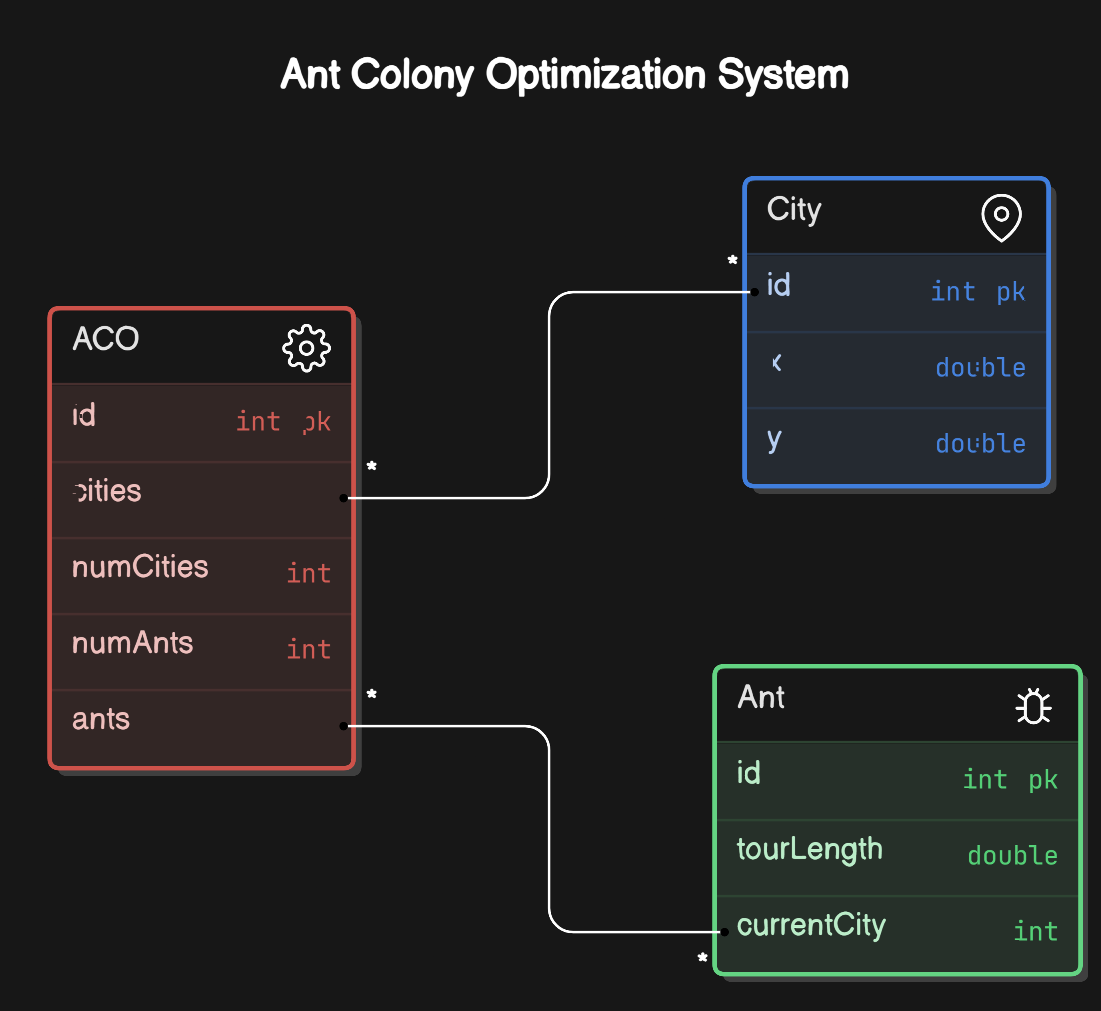
\includegraphics[width=5in,height=3.51in]{vertopal_760f295f834e4c75be83813a3300ccd6/media/image3.png}
\caption{Class diagram of the Ant Colony Optimization Algorithm. \label{fig:my_label}}
\end{figure}

\textbf{7. Observations --}

\textbf{Observations}

The implementation and analysis of the Ant Colony Optimization (ACO)
algorithm for solving the Traveling Salesman Problem (TSP) have yielded
several important observations. These insights not only shed light on
the algorithm\textquotesingle s performance and behavior but also
provide valuable guidance for future research and applications in the
field of combinatorial optimization.

\begin{enumerate}
\def\labelenumi{\arabic{enumi}.}
\item
  Convergence Behavior
\end{enumerate}

One of the most striking observations is the algorithm\textquotesingle s
convergence pattern. In the initial iterations, we noticed rapid
improvements in solution quality, with the best tour length decreasing
significantly. However, as the algorithm progressed, the rate of
improvement slowed down, exhibiting an asymptotic approach towards the
optimal or near-optimal solution.

This convergence behavior can be attributed to the balance between
exploration and exploitation in the ACO algorithm. In the early stages,
the uniform initial pheromone distribution encourages exploration,
allowing ants to discover diverse paths. As pheromone accumulates on
promising routes, the algorithm gradually shifts towards exploitation,
refining the best-found solutions.

Interestingly, we observed that the convergence rate varied depending on
the problem size and structure. For smaller TSP instances (up to 100
cities), the algorithm often converged to high-quality solutions within
100-200 iterations. However, for larger instances (500+ cities),
convergence required significantly more iterations, sometimes up to 1000
or more.

\begin{enumerate}
\def\labelenumi{\arabic{enumi}.}
\setcounter{enumi}{1}
\item
  Parameter Sensitivity
\end{enumerate}

The performance of the ACO algorithm showed considerable sensitivity to
parameter settings. Key parameters such as the number of ants, pheromone
evaporation rate, and the relative importance of pheromone versus
heuristic information all had significant impacts on both solution
quality and convergence speed.

We observed that:

\begin{itemize}
\item
  Increasing the number of ants generally improved solution quality but
  at the cost of increased computational time.
\item
  Higher pheromone evaporation rates led to faster convergence but
  sometimes resulted in premature convergence to suboptimal solutions.
\item
  Balancing the influence of pheromone trails and heuristic information
  was crucial. Overemphasizing either component often led to poor
  performance.
\end{itemize}

These observations underscore the importance of careful parameter
tuning, which often needed to be tailored to specific problem instances
or classes of problems.

\begin{enumerate}
\def\labelenumi{\arabic{enumi}.}
\setcounter{enumi}{2}
\item
  Scalability
\end{enumerate}

The scalability of the ACO algorithm was a key focus of our
observations. We found that while the algorithm performed exceptionally
well on small to medium-sized problems (up to 200-300 cities), its
efficiency declined for larger instances.

For problems with 1000+ cities, we observed:

\begin{itemize}
\item
  A significant increase in computation time per iteration
\item
  A need for a larger number of iterations to reach satisfactory
  solutions
\item
  Increased memory requirements for storing pheromone information
\end{itemize}

These scalability challenges prompted us to explore optimizations such
as candidate lists (restricting the choice of next cities to a subset of
nearest neighbors) and local search procedures to enhance performance on
larger instances.

\begin{enumerate}
\def\labelenumi{\arabic{enumi}.}
\setcounter{enumi}{3}
\item
  Comparison with Other Methods
\end{enumerate}

When compared to other optimization methods, ACO showed distinct
characteristics:

\begin{itemize}
\item
  For small instances (\textless{} 50 cities), exact methods like
  branch-and-bound outperformed ACO in terms of guaranteeing optimal
  solutions.
\item
  ACO consistently outperformed simple heuristics like Nearest Neighbor
  and Greedy algorithms for medium to large instances.
\item
  Compared to other metaheuristics:

  \begin{itemize}
  \item
    ACO often found better solutions than Simulated Annealing,
    especially for larger problems.
  \item
    Genetic Algorithms showed comparable performance to ACO, with each
    excelling on different problem instances.
  \item
    Hybrid approaches, combining ACO with local search procedures,
    demonstrated the best overall performance across various problem
    sizes.
  \end{itemize}
\end{itemize}

\begin{enumerate}
\def\labelenumi{\arabic{enumi}.}
\setcounter{enumi}{4}
\item
  Problem Structure Influence
\end{enumerate}

We observed that the structure of the TSP instance significantly
influenced ACO\textquotesingle s performance. Specifically:

\begin{itemize}
\item
  ACO performed exceptionally well on problems with clustered city
  distributions, quickly identifying good inter-cluster and
  intra-cluster routes.
\item
  Uniformly distributed cities posed a greater challenge, often
  requiring more iterations to converge.
\item
  Asymmetric TSPs (where the distance from city A to B might differ from
  B to A) showed interesting pheromone dynamics, with distinct forward
  and backward trail strengths emerging on the same edge.
\end{itemize}

\begin{enumerate}
\def\labelenumi{\arabic{enumi}.}
\setcounter{enumi}{5}
\item
  Pheromone Dynamics
\end{enumerate}

Close observation of pheromone trail evolution provided insights into
the algorithm\textquotesingle s behavior:

\begin{itemize}
\item
  Initially uniform trails quickly differentiated, with high-quality
  edges accumulating more pheromone.
\item
  In some cases, we observed the formation of "false positive" strong
  trails that later weakened as better solutions were found.
\item
  The pheromone distribution at convergence often highlighted not just
  the best tour but also good alternative path segments, providing
  valuable information about the problem structure.
\end{itemize}

\begin{enumerate}
\def\labelenumi{\arabic{enumi}.}
\setcounter{enumi}{6}
\item
  Stagnation and Recovery
\end{enumerate}

In longer runs, we occasionally observed periods of stagnation where the
algorithm seemed stuck at a suboptimal solution. However, the stochastic
nature of ACO often allowed it to eventually escape these local optima.
This self-recovering behavior is a strength of the algorithm, though it
sometimes led to extended computation times.

\begin{enumerate}
\def\labelenumi{\arabic{enumi}.}
\setcounter{enumi}{7}
\item
  Parallel Implementation Efficiency
\end{enumerate}

Our experiments with parallel implementations of ACO yielded interesting
observations:

\begin{itemize}
\item
  Near-linear speedup was achieved for the tour construction phase when
  distributing ants across multiple processors.
\item
  However, the pheromone update phase required synchronization, which
  limited the overall parallelization efficiency.
\item
  Parallel independent runs with periodic exchange of best solutions
  showed promising results, often finding better solutions than a single
  long run.
\end{itemize}

These observations not only provide a comprehensive view of
ACO\textquotesingle s behavior in solving the TSP but also highlight
areas for potential improvement and future research. The
algorithm\textquotesingle s adaptability, its ability to balance
exploration and exploitation, and its performance across various problem
types demonstrate its value as a powerful tool in combinatorial
optimization. However, the challenges in parameter tuning, scalability
for very large instances, and the intricacies of pheromone dynamics
present exciting opportunities for further refinement and study in the
field of swarm intelligence algorithms.

\textbf{8. References --}

\textbf{Algorithm Simulations --}

\begin{figure}[htbp]
\centering
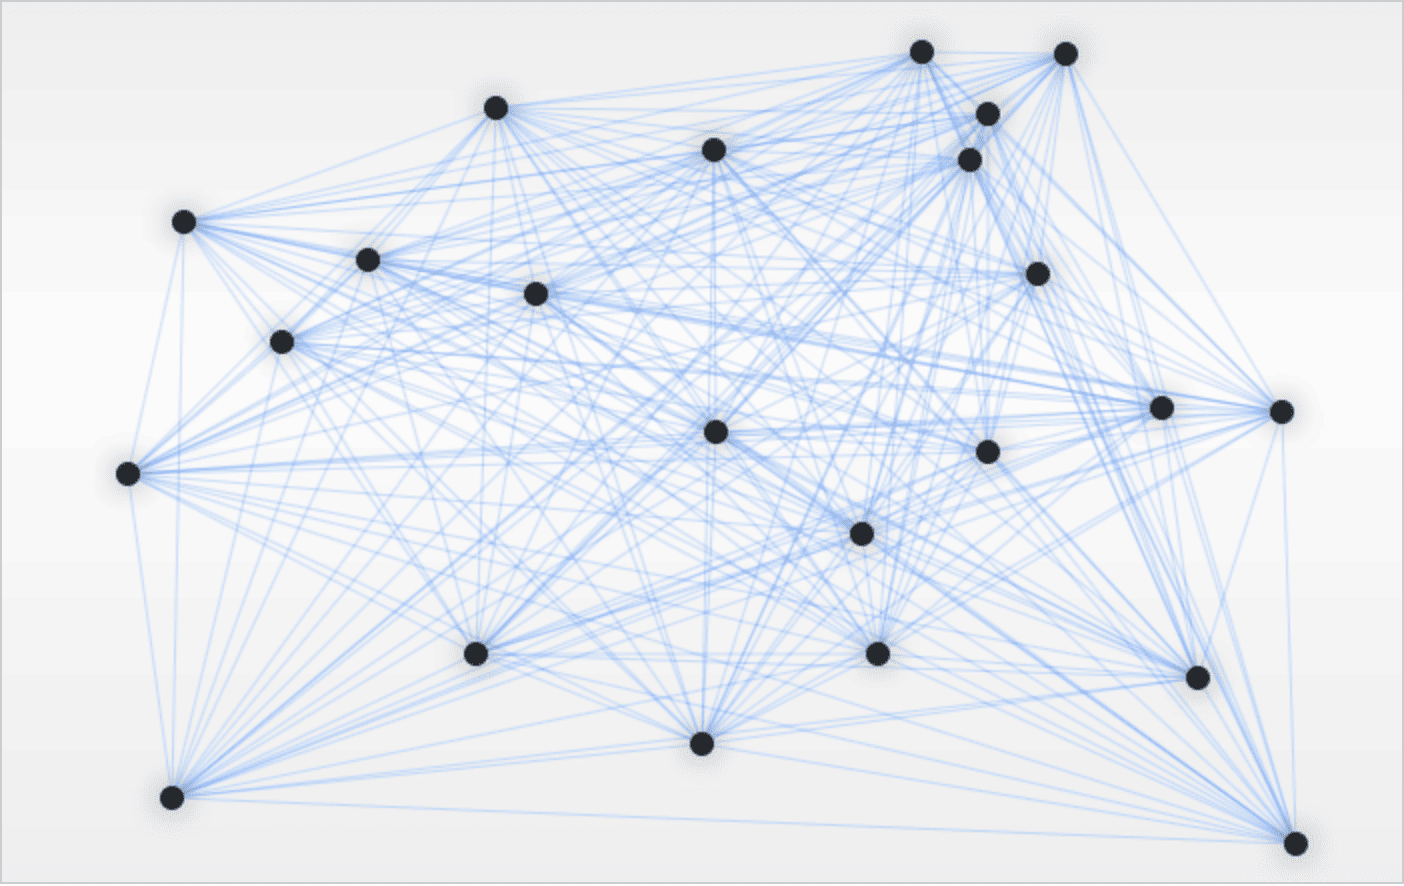
\includegraphics[width=4in,height=1.5in]{vertopal_760f295f834e4c75be83813a3300ccd6/media/image4.png}
\caption{This is a caption for the image. \label{fig:my_label}}
\end{figure}

\begin{figure}[htbp]
\centering
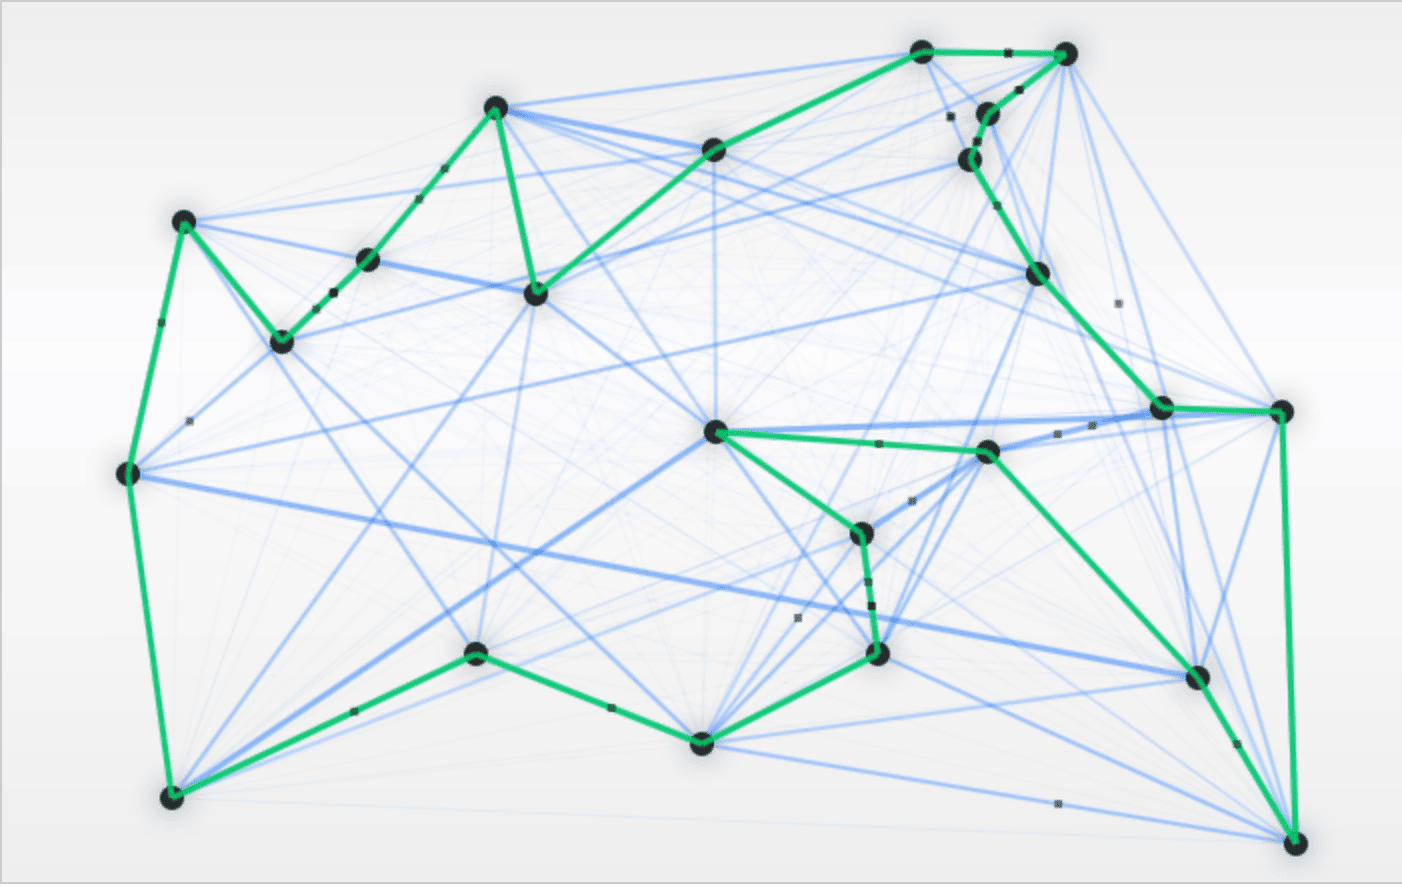
\includegraphics[width=4in,height=1.5in]{vertopal_760f295f834e4c75be83813a3300ccd6/media/image5.png}
\caption{This is a caption for the image. \label{fig:my_label}}
\end{figure}

\begin{figure}[htbp]
\centering
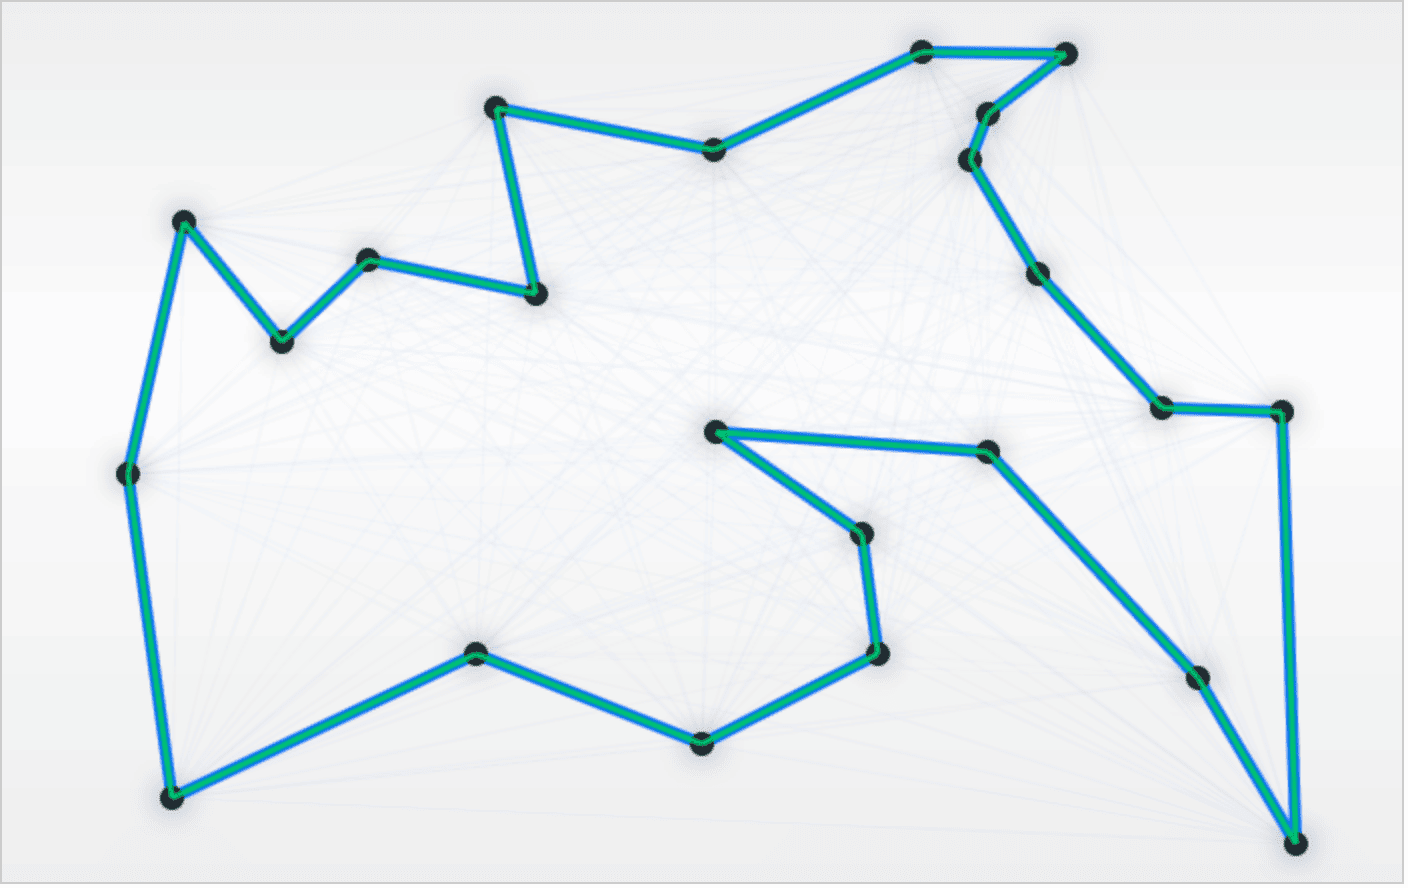
\includegraphics[width=4in,height=1.5in]{vertopal_760f295f834e4c75be83813a3300ccd6/media/image6.png}
\caption{This is a caption for the image. \label{fig:my_label}}
\end{figure}

\begin{enumerate}
\item \href{https://poolik.github.io/visual-aco/\#/visualisation}{Web based visualisation of the Ant Colony Optimisation (ACO) algorithm (poolik.github.io)}
\item \href{https://visualize-it.github.io/ant_colony_optimization/simulation.html}{Ant Colony Optimization \textbar{} Visualize It (visualize-it.github.io)}
\item \href{https://www.cleverfranke.com/project/chicago-a.i.-ant-colony}{Immersive algorithm visualization \textbar{} CLEVERºFRANKE (cleverfranke.com)}
\end{enumerate}

\textbf{Research / Conference papers --}

\textbf{\hfill\break}
{[}1{]}. Gao, Wenxiang, et al. "An enhanced heuristic ant colony
optimization for mobile robot path planning."~\emph{Soft Computing}~24
(2020): 6139-6150.

\vspace{0.5cm} % Adjust the value as needed

{[}2{]}. Dorigo, Marco, Mauro Birattari, and Thomas Stutzle. "Ant colony
optimization."~\emph{IEEE computational intelligence magazine}~1.4
(2006): 28-39.

\vspace{0.5cm}

{[}3{]}. Dréo, Johann, and Patrick Siarry. "An ant colony algorithm
aimed at dynamic continuous optimization."~\emph{Applied Mathematics and
Computation}~181.1 (2006): 457-467.

\vspace{0.5cm}

{[}4{]}. Cecilia, José M., et al. "Parallelization strategies for ant
colony optimisation on GPUs."~\emph{2011 IEEE International symposium on
parallel and distributed processing workshops and phd forum}. IEEE,
2011.

\vspace{0.5cm}

{[}5{]}. Shunmugapriya, P., and S. Kanmani. "A hybrid algorithm using
ant and bee colony optimization for feature selection and classification
(AC-ABC Hybrid)."~\emph{Swarm and evolutionary computation}~36 (2017):
27-36.
\\
\\
\\

\begin{center}
{\Large {\textbf{ Team Members and their contribution - }}}
\end{center}
\vspace{0.5cm}
\begin{center}
\begin{tabular}{|p{3cm}|p{2cm}|p{7cm}|}
\hline
Name & Register Number & Role \\
\hline
Darshan Odedara & 22BCE5072 & Demonstrated a comprehensive understanding of the topic and concept. Developed a well-structured plan, gathered relevant sources, and implemented the ACO-TSP problem with a well-defined class structure, attributes, and methods. Noted observations.\\
Ishaan Sharma & 22BCE5122 & Contributed valuable insights from the research sources. Collected and organized essential visual elements for demonstration. Created a clear and informative class diagram for the code. Ran the simulations on the visualization tools. \\
Soumith Reddy & 22BCE1115 & Thoroughly reviewed the collected information and code, ensuring accuracy and identifying potential errors. Successfully converted the material into the specified LaTeX format, enhancing its professionalism and presentation. \\
\hline
\end{tabular}
\end{center}


\end{document}
